\chapter{Polarization}

An electromagnetic wave is a transverse wave consisiting of electric and magnetic fields vibrating perpendicular to each other and to the direction of propagation.The vibrating electric field vector E and the direction of wave propagation form a plane.This plane is called plane of vibration.Now a days it is referred to as plane of polarization.
\section{Linear polarization}
 A linearly polarized light is a wave in which the electric vector oscillates in a given constant orientation.Now a days the term "linearly polarized" is more preferred and most frequently used than plane polarized.\\
 The light in which the plane of vibration are symmeytically distributed about propagation direction of the wave is known as the unpolarized light.\\
 A parallel component is represented by arrows is called \textbf{p-component}\\
 A perpedicular component is represented by dots and is called \textbf{s- component}\\
\begin{figure}[H]
	\centering
	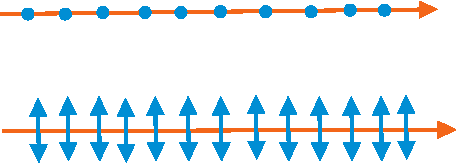
\includegraphics[height=3cm,width=5cm]{pl-crop}
	\caption{}
	\label{}
\end{figure}
 \subsection{Production of linearly polarized light}
 A plane polarized light willget from a unpolarized light in 5 different way.\\
 (I)Reflection \\
 (II)Refraction\\
 (III)Scattering\\
 (IV)Selective absorption(dichroism) \\
 (V)Double refraction\\
 \textbf{(I)Polarization by Reflection}\\
 \begin{figure}[H]
 	\centering
 	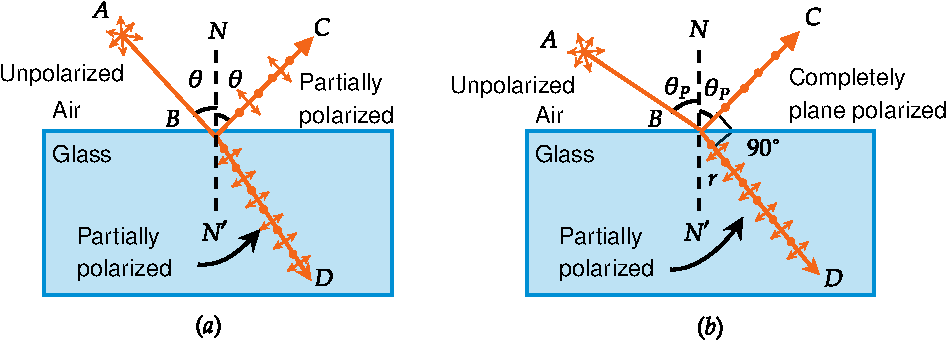
\includegraphics[height=5cm,width=12cm]{diagram-20211221(8)-crop}
 	\caption{}
 	\label{}
 \end{figure}
      When the natural light is incident on the surface ,the two components are reflected to different extent.The reflected ray has predominance of s components and as such it is partially polarized.As the angle of incidence is varied, the extend of polarization of the reflected ray varies.At a particular angle $\theta_P$ the reflection  coefficient of p component goes to zero and the reflected beam doesnot contain any p component.It contain only s component and is totally linearly polarized.The angle $\theta_p$ is called the polarizing angle or brewster's angle.\\
      The tangent of the angle at which polarization is obtained by reflection numarically equal to the refractive index of the medium.if $\theta_p$ is the angle and $\mu$ is the refractive index of the medium,then 
      $$\mu=\tan \theta_p$$
      This is known as Brewster's law.\\
      \textbf{(II)Polarization by Refraction}\\
      \begin{figure}[H]
      	\centering
      	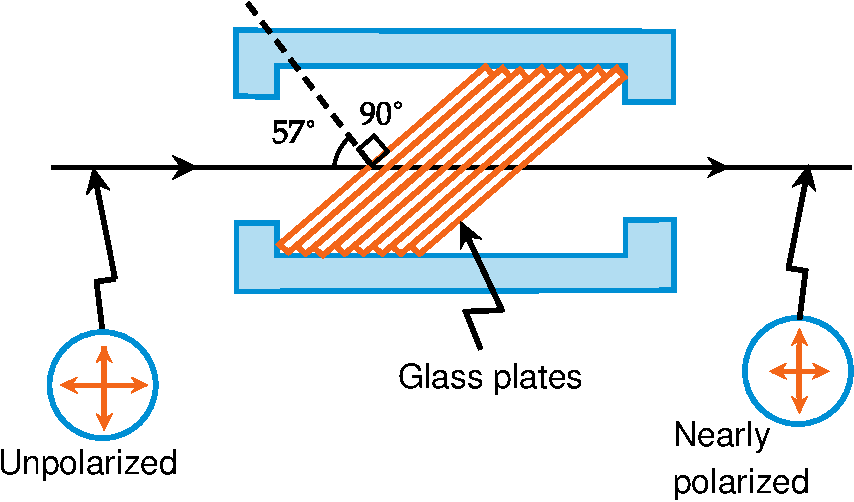
\includegraphics[height=5cm,width=10cm]{diagram-20211221(9)-crop}
      	\caption{}
      	\label{}
      \end{figure}
      When unpolarized light is incident at Brewster angle on a smooth glass surface, the reflected light is totally polarized while the refracted light is partially polarized. If natural light is transmitted through a single plate, the transmitted beam is only partially polarized. If a stack of glass plates is used instead of a single plate, reflections from successive surfaces occur leading to the filtering of the s-component in the transmitted ray. Ultimately, the transmitted ray consists of p component alone.\\
      It is found that a stack of about 15 glass plate is required for this purpose.The glass plate are supported in a tube of suitable size and are held inclined at an angle of about $33^{\circ}$ to the axix of the tube ,such an arrangements is called pile of plates.\\
      \textbf{(III)Polarization by scattering}\\
      \begin{figure}[H]
      	\centering
      	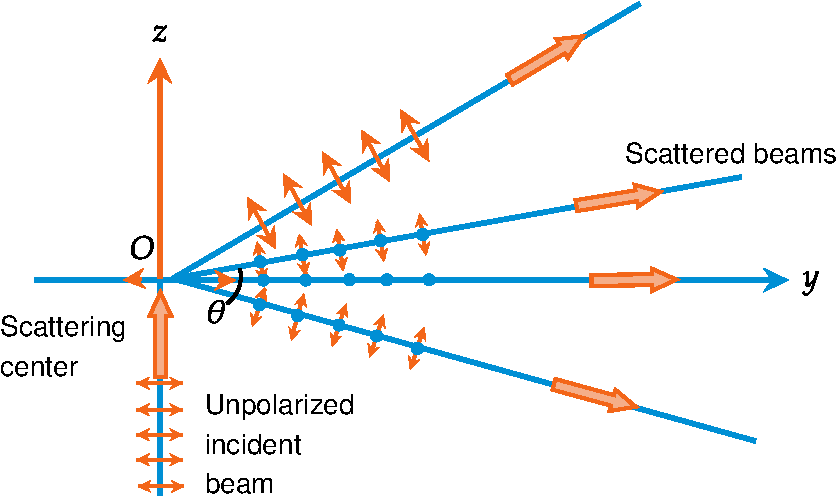
\includegraphics[height=5cm,width=8cm]{diagram-20211221(10)-crop}
      	\caption{}
      	\label{}
      \end{figure}
      If a narrow beam of natural light is incident on a transparent medium containing a suspensi of ultramicroscopic particles, the light scattered is partially polarized. The degree of polarisati depends on the angle of scattering. The beam scattered at $90^{\circ}$ with respect to the incident directi is linearly polarized. The direction of vibration of $\mathbf{E}$ vector in the scattered light will be perpendicu to the plane defined by the direction of propagation and the direction of observation.\\
      \textbf{(IV)Polarization by selective absorption}\\
     when  light passes through a crystal such as tourmaline, it is split into two components, which are polarize in mutually perpendicular planes. The crystal strongly absorbs light that is polarized in a directiv parallel to a particular plane in the crystal but freely transmits the light component polarized in perpendicular direction. This difference in the absorption for the rays is known as selective absorptio or dichroism. If the crystal is of proper thickness, one of the components is totally absorbed and the other component emerging from the crystal is linearly polarized. \\
     \textbf{(V)Polarization by double refraction}\\
     \begin{figure}[H]
     	\centering
     	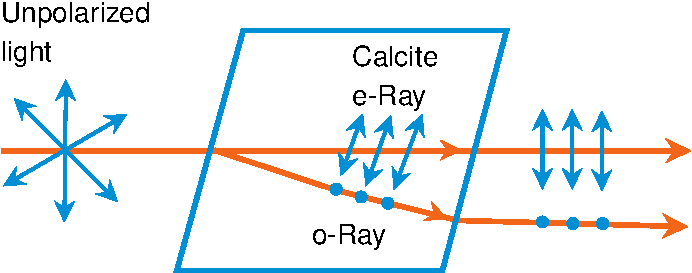
\includegraphics[height=3cm,width=5cm]{diagram-20211221(12)-crop}
     	\caption{}
     	\label{}
     \end{figure}
  When light is incident on a calcite crystal, it is split into two refracted rays differing in their properties. The phenomenon of causing two refracted rays by a crystal is called birefringence or double refraction. The crystals are said to be birefringent.\\
  Thetwo rays produced in double diffraction are linearly polarized in mutually perpedicular directions.One of the ray obeys snell's law of refraction and hence is known as an extraordinary ray or O-ray.The other ray does not obey snell's law is called extraordinary day or e-ray.Hence the two ray can be distiguished from each other.If one of the ray is eliminated ,the light transmitted by the crystal will be linearly polarized light.\\
  \textbf{Properties of o-Ray and e-Ray}
  \begin{enumerate}
  	\item Ordinary ray obeys the conventional laws of refraction
  	\item Both o-ray and e-ray are plane polarized.They are polarized in mutually perpendicular planes.The electric vector 0-ray vibrates perpendicular to the principal section of the o-ray while vibration of e-ray take place parallel to the principal section of the e-ray.
  	\item O-ray travel with the same speed in all directions with in the crystal.The e-ray travels with different speed along different direction in the crystal.However the speed of e-ray will be equal to that of o-ray along the optic axis direction.
  	\item Because 0-ray travels with the same velocity in all directions the refractive indexcorresponding to it has a constant value.On the other hand refractive index for e-ray varies from direction to direction.The refractive index of the 0-ray is defind as follows\\
  	$$\mu_{0}=\frac{c}{v_{0}}=\frac{\text { velocity of light in a vacuum }}{\text { velocity of o-ray in the crystal }}$$
  	The principal refractive index for e-ray in positive crystals is defined as follows:
  	$$
  	\mu_{e}=\frac{c}{\left(v_{e}\right)_{\min }}=\frac{\text { velocity of light in a vacuum }}{\text { minimum velocity of e-ray in the crystal }}
  	$$
  	The principal refractive index for e-ray in negative crystals is defined as follows:
  	$$
  	\mu_{e}=\frac{c}{\left(v_{e}\right)_{\max }}=\frac{\text { velocity of light in a vacuum }}{\text { maximum velocity of e-ray in the crystal }}
  	$$
  	\item When natural light is incident on an anisotropic crystal at an angle to the optic axis,it splits into o-and e-rays, which travel in different directions with different velociities
  	\item The distinction of o-ray and e-ray exists only within the crystal. Once they emerge from the crystal, they travel with the same velocity. The rays outside the crystal differ only their direction of travel and plane of polarization. The designation of o- ray and e-ray no meaning outside the crystal.
  \end{enumerate}
\subsubsection{Positive and negative crystal}
\begin{enumerate}
	\item In positive uniaxial crystals, the ellipsoid of revolution corrrsponding to the e-ray is totally contained within the sphere corresponding to the o-ray.
	In negative uniaxial crystals, the ellipsoid of revolution for e-ray lies completely outside the sphere corresponding to o-ray.
	\item In positive crystals the e-ray velocity has a maximum value along the optic axis and a minimum value in a direction perpendicular to the optic axis.
	On the other hand, in negative crystals the velocity of e-ray has a minimum value parallel to the optic axis and a maximum value in a direction perpendicular to the optic axis.
	\item In positive crystals, e-ray travels slower than o-ray in all directions except along the optic axis.
	$$
	\begin{array}{lll}
	v_{e}=v_{o} & - & \text { parallel to optic axis } \\
	v_{e}<v_{o} & - & \text { other directions }
	\end{array}
	$$
In negative crystals, o-ray travels slower than e-ray in all directions except along the optic axis.
$$v_{e}=v_{o} \quad \text { - parallel to optic axis }$$
$$v_{e}>v_{0} \quad-\quad \text { other directions }$$
\item In positive crystals the principal refractive index for e-ray is larger than the principal refractive index for o-ray.
$$\mu_{\mathrm{e}}>\mu_{\mathrm{o}}$$
In negative crystals the principal refractive index for o-ray is larger than the principal refractive index for e-ray.
$$\mu_{e}<\mu_{o}$$
\item Birefringence or amount of double refraction of a crystal is defined as
$$
\Delta \mu=\mu_{\mathrm{e}}-\mu_{\mathrm{o}}
$$
$\Delta \mu$ is a positive quantity for positive crystals as $\mu_{e}>\mu_{o}$ in these crystals.\\
 $\Delta \mu$ is a negative quantity for negative crystals as $\mu_{e}<\mu_{o}$ in these crystals.
\end{enumerate}
\subsubsection{Phase difference between e-Ray and O-ray}
When a plane polarized light wave is incident on a birefringent crystal such that its electric vector makes an angle with the optic axis, then the polarized wave splits into two polarized waves namely e-ray and o-ray. Let us consider the particular case of a slice of a positive crystal where the optic axis is parallel to refracting face of the crystal, The two waves travel along the same direction in the crystal but with different velocities. As a result, when the waves emerge from the rear face of the crystal, an optical path difference would have developed between them. The optical path difference can be calculated as follows:
Let $d$ be the thickness of the crystal.\\
$\left.\begin{array}{l}\text { The optical path for o-ray } \\ \text { within the crystal }\end{array}\right\}=\mu_{o} d$\\
$\left.\begin{array}{l}\text { The optical path for e-ray } \\ \text { within the crystal }\end{array}\right\}=\mu_{e} d$\\
$\left.\begin{array}{l}\text { The optical path difference } \\ \text { between e-ray and o -ray }\end{array}\right\} \Delta=\left(\mu_{e}-\mu_{o}\right) d$\\
Consequently, a phase difference arises between the two waves. It is given by
$$
\delta=\frac{2 \pi}{\lambda}\left(\mu_{e}-\mu_{o}\right) d
$$
\subsubsection{Super position of o-Ray and e-Ray}
\begin{enumerate}
	\item When the optical path difference is zero or even an odd multiples of $\lambda/2$ the resulting ligt wave is linearly polarized.
	\item When optical path difference $\frac{\lambda}{4}$ the resultant wave is elliptically polarized.
	\item In the particular instant when the wave amplitude are equal and the optical path difference is $\frac{\lambda}{4}$ ,the resultant wave is circularly polarized.
\end{enumerate}
\section{Quarter wave plate}
A quarter wave plate is a thin plate of birefringent crystal having the optic axis parallel to its refracting faces and its thickness adjusted such that it introduces a quarter-wave $(\lambda / 4)$ path difference (or a phase difference of $90^{\circ}$ ) between the e-ray and o-ray propagating through it.\\
When a plane polarized light wave is incident on a birefringent crystal having the optic axis parallel to its refracting face, the wave splits into e-wave and o-wave. The two waves travel along the same direction but with different velocities. As a result, when they emerge from the rear face of the crystal, an optical path difference would be developed between them. Thus, for a quartz wave plate\\
$$
\begin{aligned}
&\left(\mu_{e}-\mu_{o}\right) d=\frac{\lambda}{4} \\
&d=\frac{\lambda}{4\left[\mu_{e}-\mu_{o}\right]}
\end{aligned}
$$
A quarter wave plate introduces between e-ray and o-ray a phase difference $\delta$ given by
$$
\delta=(2 \pi / \lambda) \Delta=\pi / 2=90^{\circ}
$$
A quarter-wave plate is used in producing elliptically or circularly polarised light. It converts plane polarised light into elliptically or circularly polarised light depending upon the angle that the incident light vector makes with the optic axis of the quarter wave plate.
\section{Half wave plate}
A half wave plate is a thin plate of birefringent crystal having the optic axis parallel to refracting faces and its thickness chosen such that it introduces a half-wave $(\lambda / 2)$ path difference a phase difference of $180^{\circ}$ ) between e-ray and o-ray.\\
When a plane polarized light wave is incident on a quartz crystal having the optic axis parallel to its refracting faces, it splits into two waves: o- and e-waves. The two waves travel along the same direction inside the crystal but with different velocities. As a result, when they emerge from the rear face of the crystal, an optical path difference would be developed between them.\\
$$\begin{aligned}
	&\left(\mu_{e}-\mu_{o}\right) d=\frac{\lambda}{2} \\
	&d=\frac{\lambda}{2\left(\mu_{e}-\mu_{o}\right)}
\end{aligned}$$
$$\delta=(2 \pi / \lambda) \Delta=\pi=180^{\circ}$$
  \section{Effect of polarizer on natural light}
  \textbf{Polarizer}\\
  A polarizer is an optical device that transforms unpolarized light into polarized light.if it produces linearly polarized light it is called linear polarizer.\\
  \textbf{Analyser} \\
  Analyser is a device which is used to identify the direction of vibration of linearly polarized light.\\
  Polarizer and analyzer are fabricated in the same and have the same effect on the incident light.
         \par When unpolarized light passes through a polarizer, the intensity of the transmitted light will be exactly half that of the incident light \\
         \textit{If unpolarized light of intensity $I_0$ is incident on a polarizer,the intensity of the transmitted light through the polarizer is $\frac{I_0}{2}$}\\
         $\therefore I=\frac{I_0}{2}$
         \section{Effect of analyser on a plane polarized light-malus's law}
         \begin{figure}[H]
         	\centering
         	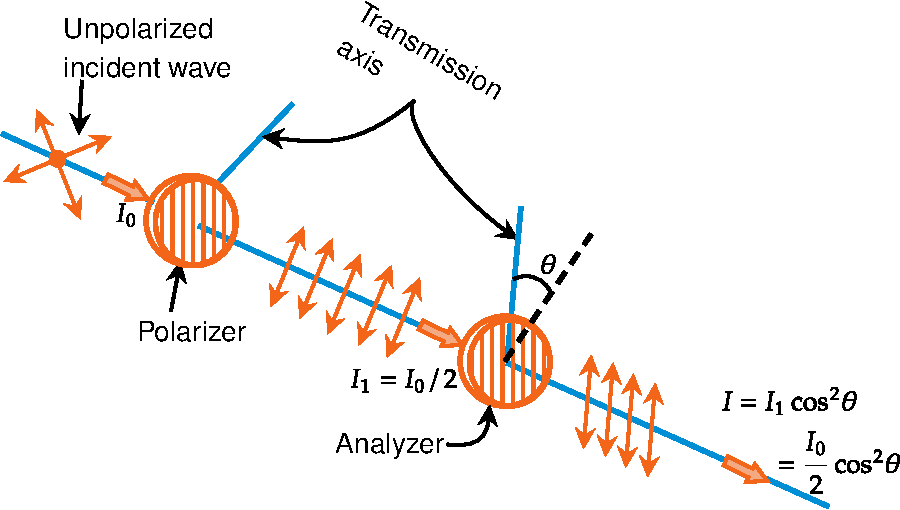
\includegraphics[height=5cm,width=10cm]{diagram-20211221(13)-crop}
         	\caption{}
         	\label{}
         \end{figure}
     When matural unpolarized light is incident on a polarizer,the transmitted light is linearly polarized.If this light passes through an analyser ,the intensity varies with the angle between the transmission axex of the polarizer and analyser.\textbf{Malus law} states that the intensity of the polarized light transmitted through the analyser is proportional to cosine square of the angle between the plane of the transmission of the analyser and the plane of transmission of the polarizer.\\
     The intensity of the light after passing through the polarizer and analyser is \\
     $$I=E^2\cos^2\theta=I_1\cos^2\theta=\frac{I_0}{2}\cos^2\theta$$
     Where $I_0$ be the initial intensity.\\
     \textbf{case (i)}if $\theta=0$\quad \quad Axes parallel  \quad \quad $I=I_1$\\\textbf{case (i)}if $\theta=0$\quad \quad Axes parallel  \quad \quad $I=I_1$\\
 \textbf{case (i)}if $\theta=180^{\circ}$\quad \quad Axes parallel \quad \quad $I=I_1$\\
 \textbf{case (i)}if $\theta=270$\quad \quad Axes perpendicular  \quad \quad $I=0$
 \begin{exercise}
 	A beam of polarized light makes angle of $60^{\circ}$ with the axis of the polaroid sheet .How much is the intensity of light transmitted through the sheet?
 \end{exercise}
\begin{answer}
	$$I=I_0\cos^2\theta$$
	$$I=I_0(\cos60)^2=\frac{1}{4}I_0$$
\end{answer}
 \section{Superposition of two linearly polarized waves}
 \textbf{(a)Superposition of two waves with parallel elctric field}\\
 Let us consider the propagation of two linearly polarized electromagnetic waves propagating along the $z$ axis) with their electric vectors oscillating along the $x$ axis. Th electric fields associated with the waves can be written in the form
 $$
 \begin{aligned}
 &E_{1}=\hat{x} a_{1} \cos \left(k z-\omega t+\theta_{1}\right) \\
 &E_{2}=\hat{x} a_{2} \cos \left(k z-\omega t+\theta_{2}\right)
 \end{aligned}
 $$
 where $a_{1}$ and $a_{2}$ represent the amplitudes of the waves, $\hat{x}$ represents the unit vector along the $x$ axis, and $\theta_{1}$ and $\theta_{2}$ are phase constants. The resultant of these two waves is given by
 $$
 E=E_{1}+E_{2}
 $$
 which can always be written in the form
 $$
 \begin{aligned}
 &E=\hat{x} a \cos (k z-\omega t+\theta) \\
 &a=\left[a_{1}^{2}+a_{2}^{2}+2 a_{1} a_{2} \cos \left(\theta_{1}-\theta_{2}\right)\right]^{\frac{1}{2}}
 \end{aligned}
 $$
represents the amplitude of the wave. Equation tells us that the resultant is also a linearly polarized wave with its electric vector oscillating along the same axis.\\
\textbf{(b)Superposition of two waves with two mutually perpendicular fields}\\
Let the two orthogonal waves be represented by
$$
\begin{aligned}
&E_{y}=E_{1} \cos (k x-\omega t) \\
&E_{z}=E_{2} \cos (k x-\omega t+\delta)
\end{aligned}
$$
$\text { The waves are of the same frequency } v=\omega / 2 \pi \text {. } \delta \text { is the phase difference between the waves. }$
 
 According to the principle of superposition
 $$
 \begin{aligned}
 E &=E_{y}+E_{z} \\
 &=E_{1} \cos (k x-\omega t)+E_{2} \cos (k x-\omega t+\delta)
 \end{aligned}
 $$
 $E_{z}=E_{2} \cos (k x-\omega t+\delta)$\\
 $\begin{aligned}
 	&E_{z}=E_{2} \cos (k x-\omega t) \cos \delta-E_{2} \sin (k x-\omega t) \sin \delta \\
 	&\quad=E_{2} \cos (k x-\omega t) \cos \delta \pm\left[1-\cos ^{2}(k x-\omega t)\right]^{1 / 2} E_{2} \sin \delta
 \end{aligned}$\\
 $E_{y}=E_{1} \cos (k x-\omega t)$\\
$ \cos (k x-\omega t)=E / E_{1}$\\
Then $E_z$ becomes\\
$$\therefore \quad E_{z}=E_{2} \frac{E_{y}}{E_{1}} \cos \delta \pm \sqrt{1-\frac{E_{y}^{2}}{E_{1}^{2}}} \quad E_{2} \sin \delta$$
Rearranging the terms, we get
$$
\left[E_{z}-\frac{E_{2}}{E_{1}} E_{y} \cos \delta\right]=\pm \sqrt{1-\left(\frac{E_{y}}{E_{1}}\right)^{2}} E_{2} \sin \delta
$$
On squaring both the sides, we obtain
$$
\begin{aligned}
&E_{z}^{2}+\frac{E_{y}^{2} E_{2}^{2}}{E_{1}^{2}} \cos ^{2} \delta-\frac{2 E_{y} E_{z} E_{2}}{E_{1}} \cos \delta=\mathrm{E}_{2}^{2} \sin ^{2} \delta-\frac{E_{y}^{2} E_{2}^{2}}{E_{1}^{2}} \sin ^{2} \delta \\
\end{aligned}
$$
Rearranging the terms ,we get
$$E_z^2+\frac{E_y^2E_2^2}{E_1^2}\left( \cos^2\delta+\sin^2\delta\right) -\frac{2E_yE_zE_2}{E_1}\cos\delta=E_2^2\sin^2\sin^2\delta$$
$$E_{z}^{2}+\frac{E_{y}^{2} E_{2}^{2}}{E_{1}^{2}}-\frac{2 E_{y} E_{z} E_{2}}{E_{1}} \cos \delta=E_{2}^{2} \sin ^{2} \delta$$
Dividing both the sides by $E_{2}^{2}$ and rearranging the terms, we obtain
$$
\frac{E_{y}^{2}}{E_{1}^{2}}+\frac{E_{z}^{2}}{E_{2}^{2}}-\frac{2 E_{y} E_{z}}{E_{1} E_{2}} \cos \delta=\sin ^{2} \delta
$$
This is the general equation of an ellipse\\
\begin{figure}[H]
	\centering
	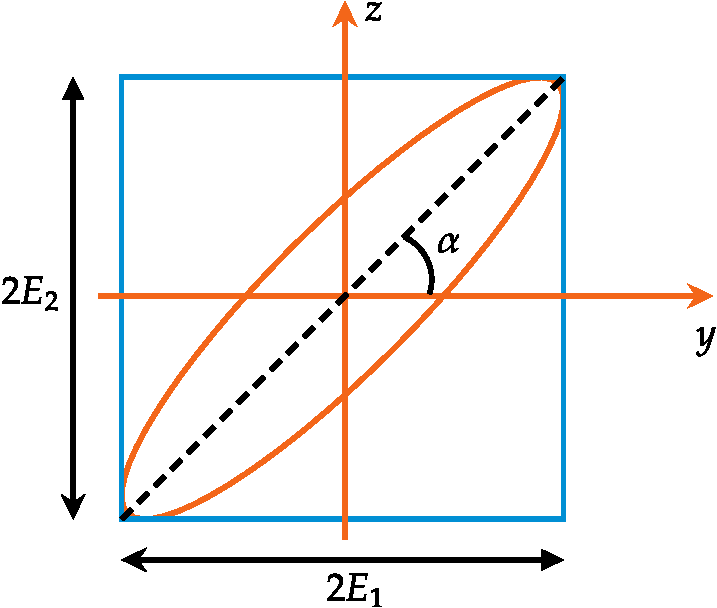
\includegraphics[height=5cm,width=8cm]{diagram-20211222(11)-crop}
	\caption{}
	\label{}
\end{figure}
\textbf{Case I}
When $\delta=0$, or $\pm 2 \mathrm{~m} \pi$, the two waves are in phase.
$\cos \delta=1$ and $\sin \delta=0$ and the equation reduces to
$$
\begin{gathered}
\frac{E_{y}^{2}}{E_{1}^{2}}+\frac{E_{z}^{2}}{E_{2}^{2}}-\frac{2 E_{y} E_{z}}{E_{1} E_{2}}=0 \\
{\left[\frac{E_{y}}{E_{1}}-\frac{E_{z}}{E_{2}}\right]^{2}=0} \\
\frac{E_{y}}{E_{1}}-\frac{E_{z}}{E_{2}}=0 \\
E_{z}=\frac{E_{2}}{E_{1}} E_{y}
\end{gathered}
$$
 The above equation represents a straight line having a slope ($\frac{E_2}{E_1}$) .It means that the resultant of two plane polarized waves, which are in phase (ie coherant waves),is again a plane polarized waves.\\
 \textbf{Case II} \\
 When $\delta=\pi$, or $\pm(2 m+1) \pi$, the two waves are in opposite phase. $\cos \delta=-1$ and $\sin \delta=0$ and the equ. (20.39) reduces to
 $$
 \begin{gathered}
 \frac{E_{y}^{2}}{E_{1}^{2}}+\frac{E_{z}^{2}}{E_{2}^{2}}-\frac{2 E_{y} E_{z}}{E_{1} E_{2}}=0 \\
 {\left[\frac{E_{y}}{E_{1}}+\frac{E_{z}}{E_{2}}\right]^{2}=0} \\
 \frac{E_{y}}{E_{1}}+\frac{E_{z}}{E_{2}}=0 \\
 E_{z}=-\frac{E_{2}}{E_{1}} E_{y}
 \end{gathered}
 $$
 This equation represents a straight line of a slope $\left(-E_{2} / E_{1}\right)$.It means that the resultant of two plane polarized waves ,which are in opposite phase(coherent waves) is again a plane polarized waves.\\
 \textbf{Case III}\\
 $\text { If } \delta=\pi / 2, \text { or } \pm(2 m+1) \pi / 2, \text { then } \cos $$\delta=0 \text { and } \sin \delta=1 . \text { Equation} \text { reduces to }$
 $$\frac{E_{y}^{2}}{E_{1}^{2}}+\frac{E_{z}^{2}}{E_{2}^{2}}=1$$
  Therefore, when the two plane polarised waves are out of phase by $90^{\circ}$, their resultant is an \textbf{elliptically polarised} wave.\\
  \textbf{Case(V)}\\
   In the particular case, when $\delta=\pi / 2$ and $E_{1}=E_{2}=E_{0}$, equation reduces to $E_{y}^{2}+E_{z}^{2}=E_{o}^{2}$
  This is the equation of a circle. Hence the resultant light is \textbf{circularly polarised.
  }
 
 \begin{figure}[H]
 	\centering
 	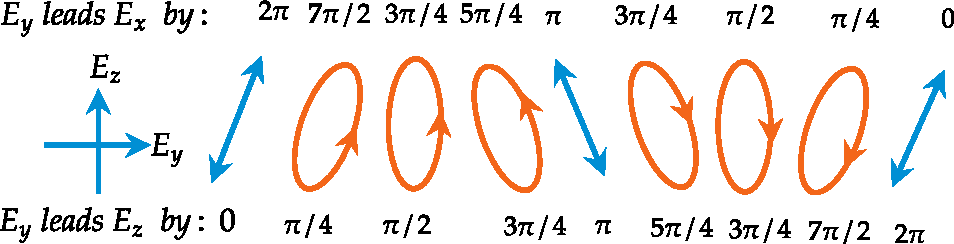
\includegraphics[height=5cm,width=15cm]{diagram-20211222(12)-crop}
 	\caption{}
 	\label{}
 \end{figure}
 
 \section{Linear polarization}
  A plane wave is linearly polarized if there is no phase difference between $E_{x}$ and $E_{y}$. We can write linear polarizations as
 $$
 \vec{E}_{0}=\left(E_{x}, E_{y}, 0\right)
 $$
 and choose the overall phase so that $E_{x}$ and $E_{y}$ are real numbers. If $E_{y}=0$ but $E_{x} \neq 0$, we have
 $$
 \vec{E}=E_{0} \hat{x} e^{i(k z-\omega t)}
 $$
 with $E_{0}=\left|\vec{E}_{0}\right|$ just a number now. Then, from Eq. (2), since $\hat{z} \times \hat{x}=\hat{y}$,
 $$
 \vec{B}=\frac{1}{c} E_{0} \hat{y} e^{i(k z-\omega t)}
 $$
 This configuration is said to be linear polarized in the $\mathrm{x}$ direction.\\
 Similarly we can have
 $$
 \vec{E}=E_{0} \hat{y} e^{i(k z-\omega t)}
 $$
 and using $\hat{z} \times \hat{y}=-\hat{x}$ :
 $$
 \vec{B}=-\frac{1}{c} E_{0} \hat{x} e^{i(k z-\omega t)}
 $$
 This configuration is said to be linear polarized in the y direction. Note that in both cases, the magnetic field is given by rotating the electric field $90^{\circ}$ counterclockwise in the $x-y$ plane and dividing by $c$.
 More generally, for any unit vector $\hat{v}$ we can have
 $$
 \vec{E}=E_{0} \hat{v} e^{i(\vec{k} \cdot \vec{x}-\omega t)}
 $$
 which is linearly polarized in the $\hat{v}$ direction. The magnetic field will be polarized in direction $90^{\circ}$ behind the electric field.
 
 Remember, we always implicitly want to have the real part of these fields. So, for linearly polarized light in the $x$ direction, the fields are actually
 $$
 \operatorname{Re}[\vec{E}]=\left(E_{0} \cos (k z-\omega t), 0,0\right), \quad \operatorname{Re}[\vec{B}]=\left(0, \frac{E_{0}}{c} \cos (k z-\omega t), 0\right)
 $$
 Note that there is no $x$ or $y$ dependence in these solutions: the fields are completely uniform in $x$ and $y$ - they are plane waves. At each point on the plane, the electric field points in the $\hat{x}$ direction with the same magnitude. This magnitude varies as we move in $z$ and in $t$ but is always uniform in the plane.
 \section{ Circular polarization}
 The components have the same magnitude but are a quarter wavelength out of phase, so $\phi_{x}-\phi_{y}=\frac{\pi}{2}$. Then,
 $$
 \vec{E}_{0}=\left(E_{0}, E_{0} e^{i \frac{\pi}{2}}, 0\right)=\left(E_{0}, i E_{0}, 0\right)
 $$
 Thus,
 $$
 \vec{E}=\left(E_{0} e^{i(k z-\omega t)}, i E_{0} e^{i(k z-\omega t)}, 0\right)
 $$
 Taking the real part gives the actual electric field
 $$
 \operatorname{Re}[\vec{E}]=\left(E_{0} \cos (k z-\omega t), \quad-E_{0} \sin (k z-\omega t), \quad 0\right)
 $$
 This is called left-handed circularly polarized light.\\
  Well, at $t=z=0$, the field is $\operatorname{Re}(\vec{E})=\left(E_{0}, 0,0\right)$ pointing in the $x$ direction. A little farther along, when $k z=\frac{\pi}{2}$, still at $t=0$, then $\operatorname{Re}(\vec{E})=\left(0,-E_{0}, 0\right)$ which points in the negative $\hat{y}$ direction. Farther along still, when $k z=\pi$, it points along $-\hat{x}$, and then $\hat{y}$ and so on. Finally, after a full wavelength, it goes back to $\hat{x}$. Thus, as we move along $z$, the polarization rotates clockwise in the $x-y$ plane. Equivalently, at a given $z$, as time progresses it also rotates in the $x-y$ plane.\\
 $\begin{aligned}
 	\text { Similarly, taking } \phi_{x}-\phi_{y} &=-\frac{\pi}{2} \text { gives } \vec{E}_{0}=\left(E_{0},-i E_{0}, 0\right) \\
 	\operatorname{Re}[\vec{E}] &=\left(E_{0} \cos (k z-\omega t), E_{0} \sin (k z-\omega t), 0\right)
 \end{aligned}$\\
 which is right-handed circularly polarized light. In this case, at $t=0$ and $k z=0$, the polarization points in the $\hat{x}$ direction. A quarter wavelength farther, it points in the $\hat{y}$ direction, and so one. So this field rotates counterclockwise in the $x-y$ plane.\\
 Note that when we add left and right handed polarizations we get
 $$
 \vec{E}_{0}=\left(E_{0}, i E_{0}, 0\right)+\left(E_{0},-i E_{0}, 0\right)=\left(2 E_{0}, 0,0\right)
 $$
 which is linearly polarized in the $\hat{x}$ direction. Similarly, subtracting them gives linear polarization in the $\hat{y}$ direction. Thus circular and linear polarizations are not linearly independent. Indeed, any possible polarization can be written as a linearly combination of left-handed and right-handed circularly polarized light.
 \begin{note}
 	Circularly polarized light has angular momentum $\pm \mathrm{e}_{0}|\vec{E}|^{2} \hat{k}$, with the positive sign for lefthanded and the negative sign for right-handed. Linearly polarized light carries no angular momentum. This is easy to understand because it is a sum of left and right handed light.
 \end{note}
\section{elliptical polarization.}
 we can consider also varying the magnitudes of the different components and the phase. The most general parameterization is
 $$\vec{E}_{0}=E_{x} \hat{x} \cos (k z-\omega t)+E_{y} \hat{y} \cos (k z-\omega t+\phi)$$

 When $E_{x}$ and $E_{y}$ are different and the relative phase $\phi$ is nonzero, the polarization changes in magnitude as it rotates in the $x-y$ plane. It thereby describes an ellipse, and this is called elliptical polarization. Linear polarization corresponds to $\phi=0$. Circular polarization corresponds to $\phi=\pm \frac{\pi}{2}$ and $E_{x}=E_{y}$.
 
 
 
 
 
 
 
 
 
 
 
 
 
 
 
 
 
 
 
 
 
 
 
 
 
 
 
 
 
 
 
 
 
 
 
 
 
 
 
 
 
 
 
 
 
 
 
 
 
 
 
 
 
 
 
 
 
 
 
 
 
 
 
 
 
 
\begin{minipage}{0.33\textwidth}
	\begin{figure}[H]
		\begin{center}
			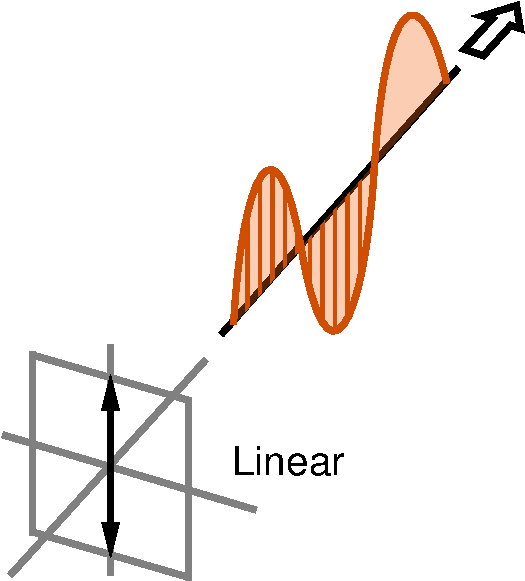
\includegraphics[width=0.7\textwidth]{linear2}
		\end{center}
	\end{figure}
\end{minipage}
\begin{minipage}{0.33\textwidth}
	\begin{figure}[H]
		\begin{center}
			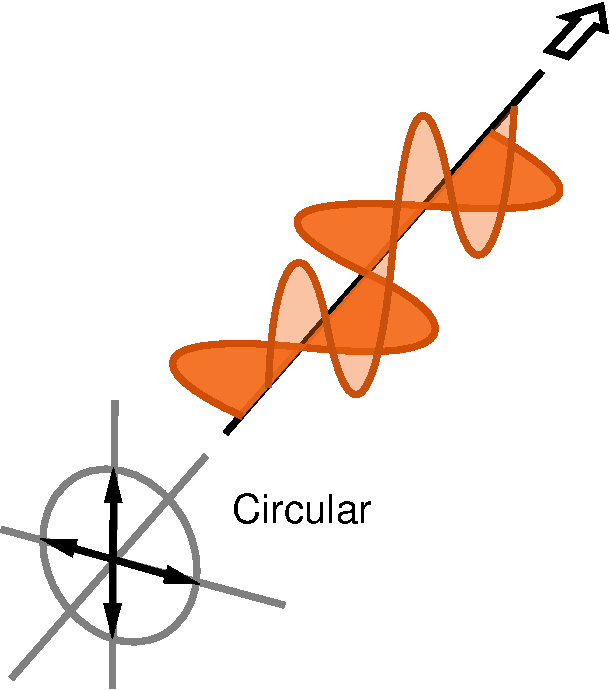
\includegraphics[width=0.7\textwidth]{circular2}
		\end{center}
	\end{figure}
\end{minipage}
\begin{minipage}{0.33\textwidth}
	\begin{figure}[H]
		\begin{center}
			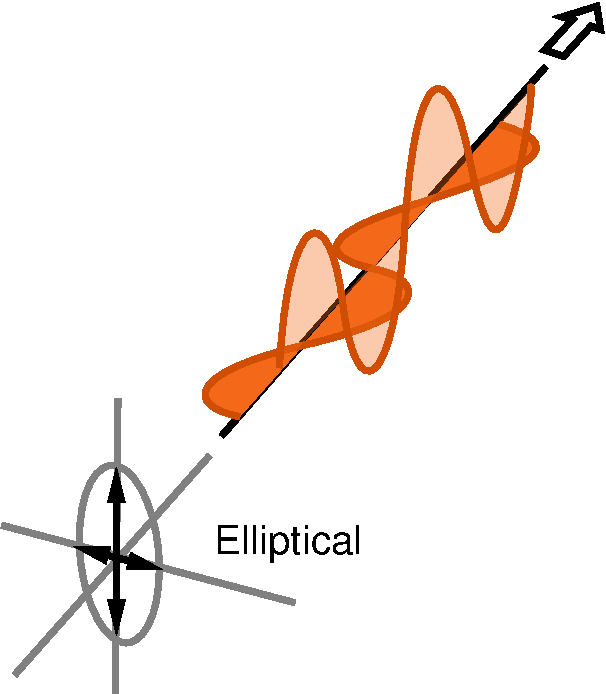
\includegraphics[width=0.7\textwidth]{elliptical2}
		\end{center}
	\end{figure}
\end{minipage}
\section{Production of elliptically polarized light}
\begin{figure}[H]
	\centering
	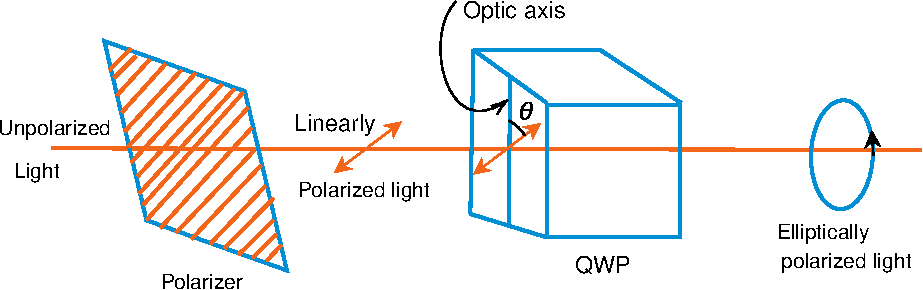
\includegraphics[height=5cm,width=12cm]{ely2(1)-crop}
	\caption{}
	\label{}
\end{figure}
Unpolarized light is first converted in to plane polarized light by allowing it to pass through the polarizer.The plane polarized light is then made incident on a quarter wave plate.The quarter wave plate or the polarizer is rotated such that the elcetric vector E 
of the plane polarized light wave make an angle $\theta\neq45^{\circ}$ with optic axis of the quarter wave plate.The incident ray divides into o-ray and e-ray of amplitude E$\sin\theta$ and E$\cos\theta$.The ray travels along the same direction in the crystal with different velocities.The two rays are polarized in orthogonal planes.They are in phase at the front phase but progressevely get out of phase as they travels through the crystal.When they emerge out of the crystal they will have a path difference of $\lambda/4$ or phase difference of $90^{\circ}$
\subsection{Detection of elliptically polarized light}
\begin{figure}[H]
	\centering
	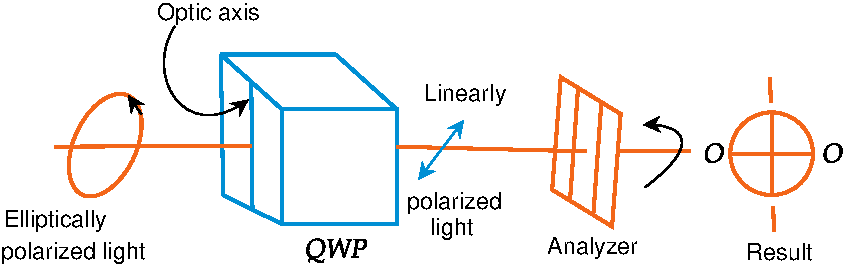
\includegraphics[height=5cm,width=12cm]{detection-crop}
	\caption{}
	\label{}
\end{figure}
A light beam is allowed to pass through an analyzer .If on rotating the analyzer the intensity of the emerging beam varies from a maximum to minimum value  but it never zero,then the incident light is elliptically polarized.The two case may be distiguished by inserting a quarter wave plate in the path of the light before it falls on the analyzer.If the original light is elliptically polarized ,it may be considered as resultant of two coherent plane polarized waves that is e-ray and o-ray.which are out of phase by $90^{\circ}$.If the light passes through the quarter wave plate an additional phase difference  $90^{\circ}$ is introduced e-ray and o-ray.THerefore the total phase difference becomes $180^{\circ}$ between the e-ray and o-ray.On emerging from the quarter plate,the e-ray and o-ray combine to produce plane polarized light.The light coming out of the QWP is examined with an analyzer the light is extiguished twice in one full rotation of the polarizer.
\section{Production of circularly polarized light}
\begin{figure}[H]
	\centering
	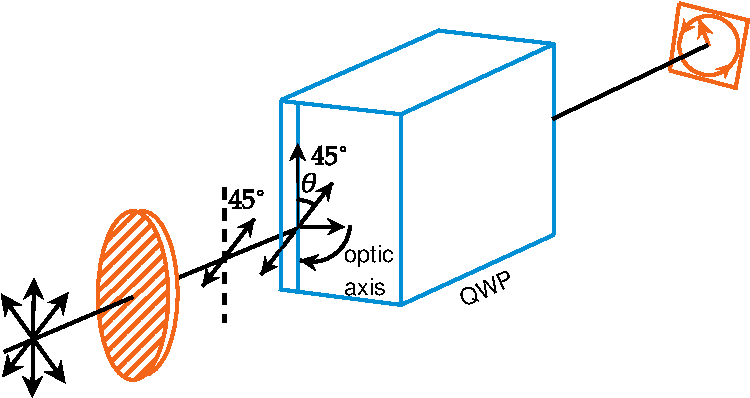
\includegraphics[height=5cm,width=12cm]{diagram-20211224(5)-crop}
	\caption{}
	\label{}
\end{figure}
Unpolarized light is first converted to plane poalrized light by allowing it to pass through a polarizer.Plane polarized light is then made to be incident on a quarter wave plate.The polarizer and quarter wave plate arerotated such that electric vector E of the plane polarized wave make an angle $45^{\circ}$ with the optic axis of quarter wave plate.The plane polarized light incident on the quarter wave plate splits in to two rays e-ray and 0-ray of equal amplitude.THe two rays travels in the same direction inside the crystal but different velocities.The two rays are in phase at the front face of the crystal but progressively get out of phase as they travel through the crystal.As they emerge from the rear face of the crystal they will have a path difference of $\lambda/4$ or phase difference of $90$.THe two rays are linearly polarized in mutually perpendicular durections.When they combine they will produce circularly polarized light.
\subsection{Detection of circularly polarized light}
\begin{figure}[H]
	\centering
	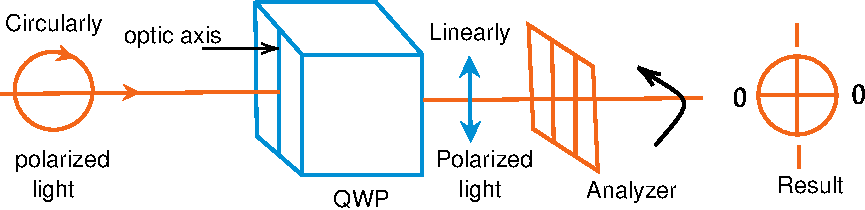
\includegraphics[height=3cm,width=12cm]{detect-crop}
	\caption{}
	\label{}
\end{figure}
The light beam is allowed to pass through an analyser (a polaroid sheet or a Nicol prism). If on rotating the analysing polaroid sheet or Nicol, the intensity of the emerging beam remains uniform, then the incident light is circularly polarized. A similar result would be obtained if the incident light is ordinary unpolarized light. The two cases may be distinguished by inserting a quarter wave plate in the path of light before it falls on the analyser. If the given light is circularly polarized, it may be considered as resultant of two coherent plane polarized waves, that is e-ray and o-ray, which are out of phase by $90^{\circ}$. If the light passes through the quarter wave plate, an additional phase difference of $90^{\circ}$ is introduced between the e-ray and o-ray. Therefore, the total phase difference becomes $180^{\circ}$ between the e-ray and o-ray. On emerging from the quarter plate, the e- and o-rays combine to produce plane polarized light. Therefore, if the light coming out of quarter wave plate is examined with an analyser, light will be extinguished twice in one full rotation of the polarizer as shown in Figure.\\
\newpage 
\begin{abox}
	Practice set 1
	\end{abox}

\begin{enumerate}
\begin{minipage}{\textwidth}
	\item $\text { Consider three polarizer's } P_{1}, P_{2} \text { and } P_{3} \text { placed along an axis as shown in the figure. }$\\
	\begin{figure}[H]
		\centering
		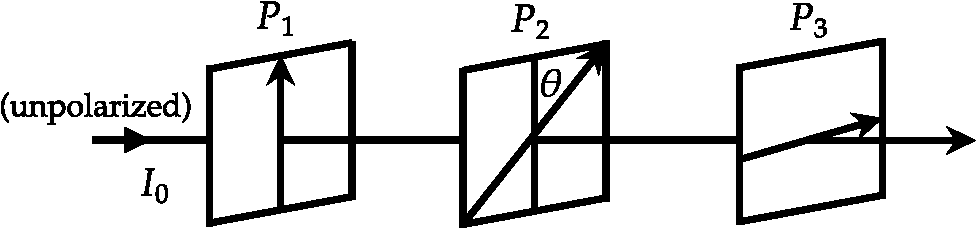
\includegraphics[height=3cm,width=9cm]{diagram-20211011(8)-crop}
	\end{figure}
	The pass axis of $P_{1}$ and $P_{3}$ are at right angles to each other while the pass axis of $P_{2}$ makes an angle $\theta$ with that of $P_{1}$. A beam of unpolarized light of intensity $I_{0}$ is incident on $P_{1}$ as shown. The intensity of light emerging from $P_{3}$ is
	\exyear{NET 2011}
\end{minipage}
\begin{tasks}(2)
	\task[\textbf{A.}]0
	\task[\textbf{B.}] $\frac{I_{0}}{2}$
	\task[\textbf{C.}]$\frac{I_{0}}{8} \sin ^{2} 2 \theta$
	\task[\textbf{D.}]$\frac{I_{0}}{4} \sin ^{2} 2 \theta$
\end{tasks}
\begin{minipage}{\textwidth}
	\item A beam of unpolarized light in a medium with dielectric constant $\in_{1}$ is reflected from a plane interface formed with another medium of dielectric constant $\in_{2}=3 \in_{1}$. The two media have identical magnetic permeability. If the angle of incidence is $60^{\circ}$, then the reflected light
	\exyear{NET 2015}
\end{minipage}
\begin{tasks}(1)
	\task[\textbf{A.}] is plane polarized perpendicular to the plane of incidence
	\task[\textbf{B.}] is plane polarized parallel to the plane of incidence
	\task[\textbf{C.}]is circularly polarized
	\task[\textbf{D.}] has the same polarization as the incident light
\end{tasks}
\begin{minipage}{\textwidth}
	\item The electric field of an electromagnetic wave is
	$$
	\vec{E}(z, t)=E_{0} \cos (k z+\omega t) \hat{i}+2 E_{0} \sin (k z+\omega t) \hat{j}
	$$
	where $\omega$ and $k$ are positive constants. This represents
	\exyear{NET 2016}
\end{minipage}
\begin{tasks}(1)
	\task[\textbf{A.}] a linearly polarised wave travelling in the positive $z$-direction
	\task[\textbf{B.}]a circularly polarised wave travelling in the negative $z$-direction
	\task[\textbf{C.}]an elliptically polarised wave travelling in the negative $z$-direction
	\task[\textbf{D.}] an unpolarised wave travelling in the positive $z$-direction
\end{tasks}
\end{enumerate}
\colorlet{ocre1}{ocre!70!}
\colorlet{ocrel}{ocre!30!}
\setlength\arrayrulewidth{1pt}
\begin{table}[H]
	\centering
	\arrayrulecolor{ocre}
	
	\begin{tabular}{|p{1.5cm}|p{1.5cm}||p{1.5cm}|p{1.5cm}|}
		\hline
		\multicolumn{4}{|c|}{\textbf{Answer key}}\\\hline\hline
		\rowcolor{ocrel}Q.No.&Answer&Q.No.&Answer\\\hline
		1&\textbf{c}&2&\textbf{a}\\\hline
		3&\textbf{c}&&\\\hline
	\end{tabular}
\end{table}
\newpage
\begin{abox}
	Practice set 2
	\end{abox}
\begin{enumerate}
\begin{minipage}{\textwidth}
	\item A circularly polarized monochromatic plane wave is incident on a dielectric interface at Brewaster angle. Which one of the following statements is correct?
	\exyear{GATE 2013}
\end{minipage}
\begin{tasks}(1)
	\task[\textbf{A.}] The reflected light is plane polarized in the plane of incidence and the transmitted light is circularly polarized.
	\task[\textbf{B.}]The reflected light is plane polarized perpendicular to the plane of incidence and the transmitted light is plane polarized in the plane of incidence.
	\task[\textbf{C.}]The reflected light is plane polarized perpendicular to the plane of incidence and the transmitted light is elliptically polarized.
	\task[\textbf{D.}]There will be no reflected light and the transmitted light is circularly polarized.
\end{tasks}
\begin{minipage}{\textwidth}
	\item An unpolarized light wave is incident from air on a glass surface at the Brewster angle. The angle between the reflected and the refracted wave is
	\exyear{GATE 2014}
\end{minipage}
\begin{tasks}(2)
	\task[\textbf{A.}] $0^{\circ}$
	\task[\textbf{B.}]$45^{\circ}$
	\task[\textbf{C.}]$90^{\circ}$
	\task[\textbf{D.}]$120^{\circ}$
\end{tasks}
\begin{minipage}{\textwidth}
	\item A plane wave $(\hat{x}+i \hat{y}) E_{0} \exp [i(k z-\omega t)]$ after passing through an optical element emerges as $(\hat{x}-i \hat{y}) E_{0} \exp [i(k z-\omega t)]$, where $k$ and $\omega$ are the wavevector and the angular frequency, respectively. The optical element is a
	\exyear{GATE 2015}
\end{minipage}
\begin{tasks}(2)
	\task[\textbf{A.}] quarter wave plate
	\task[\textbf{B.}] half wave plate
	\task[\textbf{C.}] polarizer
	\task[\textbf{D.}]Faraday rotator
\end{tasks}
\begin{minipage}{\textwidth}
	\item A quarter wave plate introduces a path difference of $\lambda / 4$ between the two components of polarization parallel and perpendicular to the optic axis. An electromagnetic wave with $\vec{E}=(\hat{x}+\hat{y}) E_{0} e^{i(k z-\omega t)}$ is incident normally on a quarter wave plate which has its optic axis making an angle $135^{\circ}$ with the $x$-axis as shown. The emergent electromagnetic wave would be
	\exyear{GATE 2018}
	\begin{figure}[H]
		\centering
		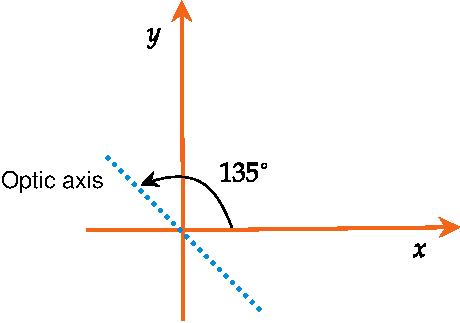
\includegraphics[height=4cm,width=6cm]{143-crop}
	\end{figure}
\end{minipage}
\begin{tasks}(1)
	\task[\textbf{A.}] elliptically polarized
	\task[\textbf{B.}]circularly polarized
	\task[\textbf{C.}]linearly polarized with polarization as that of incident wave
	\task[\textbf{D.}]linearly polarized but with polarization at $90^{\circ}$ to that of the incident wave
\end{tasks}
\begin{minipage}{\textwidth}
	\item The electric field of an electromagnetic wave is given by $\vec{E}=3 \sin (k z-\omega t) \hat{x}+$ $4 \cos (k z-\omega t) \hat{y}$. The wave is
	\exyear{GATE 2019}
\end{minipage}
\begin{tasks}(1)
	\task[\textbf{A.}] linearly polarized at an angle $\tan ^{-1}\left(\frac{4}{3}\right)$ from the $x$-axis
	\task[\textbf{B.}]linearly polarized at an angle $\tan ^{-1}\left(\frac{3}{4}\right)$ from the $x$-axis
	\task[\textbf{C.}] elliptically polarized in clockwise direction when seen travelling towards the observer
	\task[\textbf{D.}] elliptically polarized in counter-clockwise direction when seen travelling towards the observer
\end{tasks}
\begin{minipage}{\textwidth}
	\item In a set of $N$ successive polarizers, the $m^{\text {th }}$ polarizer makes an angle $\left(\frac{m \pi}{2 N}\right)$ with the vertical. A vertically polarized light beam of intensity $I_{0}$ is incident on two such sets with $N=N_{1}$ and $N=N_{2}$, where $N_{2}>N_{1} .$ Let the intensity of light beams coming out be $I\left(N_{1}\right)$ and $I\left(N_{2}\right)$, respectively. Which of the following statements is correct about the two outgoing beams?
	\exyear{GATE 2019}
\end{minipage}
\begin{tasks}(1)
	\task[\textbf{A.}] $I\left(N_{2}\right)>I\left(N_{1}\right) ;$ the polarization in each case is vertical
	\task[\textbf{B.}]$I\left(N_{2}\right)<I\left(N_{1}\right)$; the polarization in each case is vertical
	\task[\textbf{C.}]$I\left(N_{2}\right)>I\left(N_{1}\right)$; the polarization in each case is horizontal
	\task[\textbf{D.}]$I\left(N_{2}\right)<I\left(N_{1}\right)$; the polarization in each case is horizontal
\end{tasks}
\begin{minipage}{\textwidth}
	\item When unpolarised light is incident on a glass plate at a particular angle, it is observed that the reflected beam is linearly polarized. What is the angle of the refracted beam with respect to the surface normal?
	\exyear{JEST 2012}
\end{minipage}
\begin{tasks}(1)
	\task[\textbf{A.}] $56.7^{0}$
	\task[\textbf{B.}]$33.4^{0}$
	\task[\textbf{C.}]$23.3^{0}$
	\task[\textbf{D.}]The light is completely reflected and there is no refracted beam.
\end{tasks}
\begin{minipage}{\textwidth}
	\item $\text { The electric field } \vec{E}=E_{0} \sin (\omega t-k z) \hat{x}+2 E_{0} \sin \left(\omega t-k z+\frac{\pi}{2}\right) \hat{y} \text { represents: }$
	\exyear{JEST 2016}
\end{minipage}
\begin{tasks}(1)
	\task[\textbf{A.}] a linearly polarized wave
	\task[\textbf{B.}]a right-hand circularly polarized wave
	\task[\textbf{C.}]a left-hand circularly polarized wave
	\task[\textbf{D.}]an elliptically polarized wave
\end{tasks}
\end{enumerate}
\colorlet{ocre1}{ocre!70!}
\colorlet{ocrel}{ocre!30!}
\setlength\arrayrulewidth{1pt}
\begin{table}[H]
	\centering
	\arrayrulecolor{ocre}
	
	\begin{tabular}{|p{1.5cm}|p{1.5cm}||p{1.5cm}|p{1.5cm}|}
		\hline
		\multicolumn{4}{|c|}{\textbf{Answer key}}\\\hline\hline
		\rowcolor{ocrel}Q.No.&Answer&Q.No.&Answer\\\hline
		1&\textbf{c}&2&\textbf{c}\\\hline
		3&\textbf{b}&4&\textbf{c}\\\hline
		5&\textbf{d}&6&\textbf{c}\\\hline
		7&\textbf{b}&8&\textbf{d}\\\hline
	\end{tabular}
\end{table}





































